\documentclass[10pt,a4paper]{article}
\usepackage[latin1]{inputenc}
\usepackage{amsmath}
\usepackage{amsfonts}
\usepackage{amssymb}
\usepackage{graphicx}
\usepackage{float}

\usepackage{caption}
\usepackage{subcaption}

\begin{document}

\section{February 29th 2016}
\begin{itemize}
\item Show the area with a colorbar showing height
\item Fix problem with z-values close to infinity or below zero
\item Look at the spill point analysis for the area after lowering the terrain at all places where there are lakes
\end{itemize}

\subsection{Overview of the landscape that we have data over}
\begin{figure*}[h!]
    \centering
    \begin{subfigure}[h]{0.65\textwidth}
        \centering
        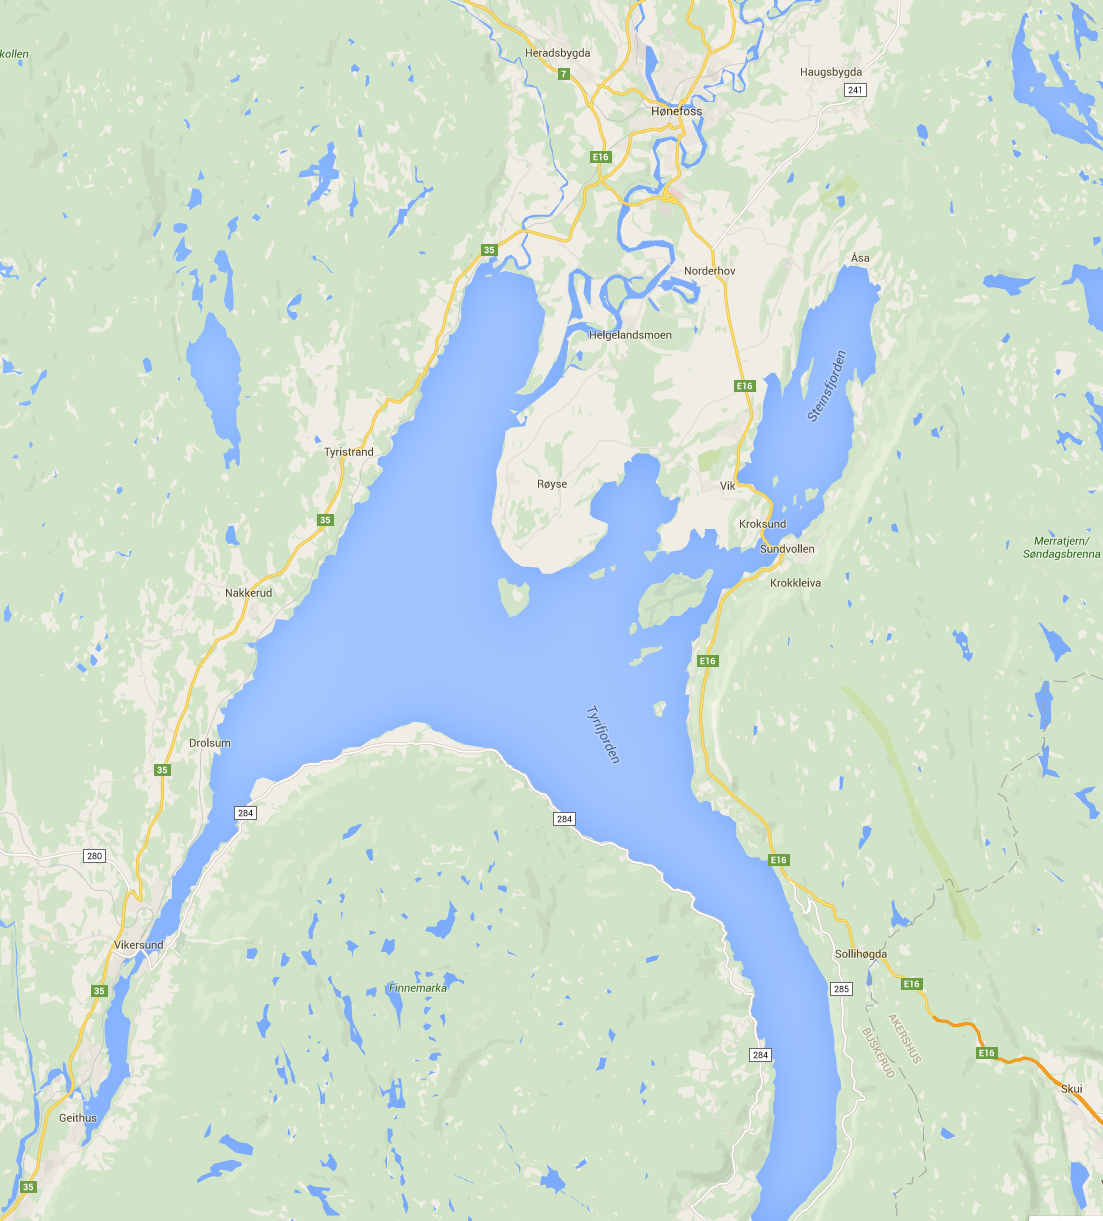
\includegraphics[height=1\textwidth]{map_area.png}
        \caption{The landscape as seen in Google Maps.}
    \end{subfigure}%
    ~ 
    \begin{subfigure}[h]{0.65\textwidth}
        \centering
        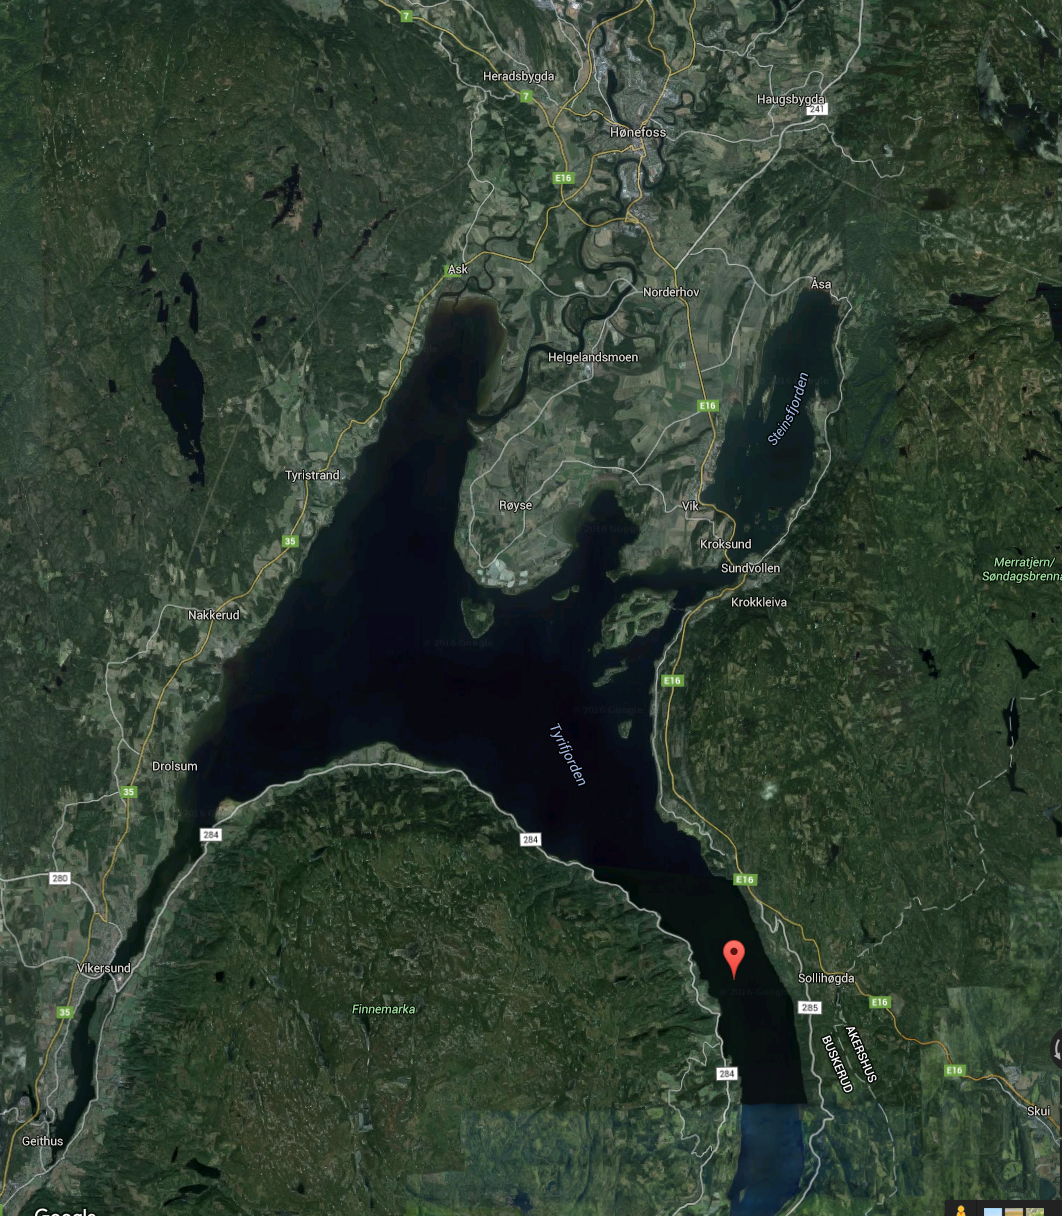
\includegraphics[height=1\textwidth]{earth_map.png}
        \caption{The landscape as seen in Google Earth.}
    \end{subfigure}
    \caption{Two different views of the landscape.}
\end{figure*}

\begin{figure}[H]
  \centering
    \includegraphics[width=1.1\textwidth]{landscape_hoh.eps}
  \caption{The landscape with height shown. Black is 0 meters above sea level. White is 1200 masl.}
\end{figure}

\subsection{Problem: z-values close to infinity or below zero}
For a given area we have a matrix $z$ which gives the height for some coordinate in the area. In some cases there might be $z$-values which for some reason are clearly wrong, e.g. the value is larger than the tallest point in Norway. In those cases we need to remove them. One way of doing this is the one below.
\begin{align}
zvals(zvals > 2469) = \textrm{NaN}\\
zvals(zvals < 0) = \textrm{NaN}\\
zvals = inpaint\_nans(double(zvals))
\end{align}
All $z$-values larger than a threshold will be set to NaN and given as input to a function that finds NaN-elements in a matrix and interpolates them with neighboring points. The function can be found in the link below:\\
 http://www.mathworks.com/matlabcentral/fileexchange/4551-inpaint-nans


\subsection{Lowering the terrain at the points where we know there are rivers}
The idea is that we can improve the spill point analysis by lowering the terrain at all points where we know there is a lake. This is given from the anders\_innsjo.tiff file, which has a bool for every point indicating whether or not there is a lake at the coordinate. Lowering the terrain by 20 meters for these points, with a downsampling factor of 8, yields the figure \ref{fig:lowered_20m_dsfac8}. Lowering by 100 meters results in figure \ref{fig:lowered_100m_dsfac8}.

\begin{figure}[H]
  \centering
    \includegraphics[width=1.2\textwidth]{reduced_height_20m_dsfacf8.eps}
  \caption{Spill point analysis after lowering lakes by 20 meters. Dsfac = 8}
  \label{fig:lowered_20m_dsfac8} 
\end{figure}

\begin{figure}[H]
  \centering
    \includegraphics[width=1.2\textwidth]{reduced_height_100m_dsfacf8.eps}
  \caption{Spill point analysis after lowering lakes by 100 meters. Dsfac = 8}
  \label{fig:lowered_100m_dsfac8}
\end{figure}

\section{March 2nd 2016}
\begin{itemize}
\item Fix problem with negative heights after lowering
\end{itemize}


\section{March 4th 2016}
\begin{itemize}
\item Fix inverted z-axis in plot
\end{itemize}

After fixing the inverted z-axis in the plots, we now yield the solutions in figure \ref{fig:trap_analysis_overview_20m_df8} and figure \ref{fig:trap_analysis_traps_20m_df8}.

\begin{figure}[H]
  \centering
    \includegraphics[width=0.8\textwidth]{20m_df8_lakes_bigrivers_overview.pdf}
  \caption{Spill point analysis after lowering lakes by 20 meters. Dsfac = 8. Included here are lakes and big rivers.}
  \label{fig:trap_analysis_overview_20m_df8}
\end{figure}

\begin{figure}[H]
  \centering
    \includegraphics[width=0.8\textwidth]{20m_df8_lakes_bigrivers.pdf}
  \caption{Spill point analysis after lowering lakes by 20 meters. Dsfac = 8. Included here are lakes and big rivers.}
  \label{fig:trap_analysis_traps_20m_df8}
\end{figure}

When doing the same for 100 meters we obtain figure \ref{fig:trap_analysis_traps_100m_df8}.

\begin{figure}[H]
  \centering
    \includegraphics[width=0.5\textwidth]{100m_df8_lakes_bigrivers.pdf}
  \caption{Spill point analysis after lowering lakes by 100 meters. Dsfac = 8. Included here are lakes and big rivers.}
  \label{fig:trap_analysis_traps_100m_df8}
\end{figure}

\section{March 6th 2016}
\begin{itemize}
\item MRST in Python?
\item Need to localize watersheds for a region and look at the size of the area
\item Combine above information with the amount of precipitation for a region
\item Include information about infiltration into groundwater
\item Include information about how long time it will take for a water particle to reach the river from a given point in the watershed
\end{itemize}


\end{document}